\documentclass{beamer}
\usepackage{ctex, hyperref}
\usepackage[T1]{fontenc}

% other packages
\usepackage{latexsym,amsmath,xcolor,multicol,booktabs,calligra}
\usepackage{graphicx,pstricks,listings,stackengine,newtxtext,newtxmath,tikz,caption,subcaption,pgfplots}



\author{赵万春}
\title{信息设计导论}
\subtitle{贝叶斯劝说框架与进展}
\institute{天津财经大学 金融学院}
\date{2024年5月24日}
\usepackage{tufe}

% defs
\def\cmd#1{\texttt{\color{red}\footnotesize $\backslash$#1}}
\def\env#1{\texttt{\color{blue}\footnotesize #1}}
\definecolor{deepblue}{rgb}{0,0,0.5}
\definecolor{deepred}{rgb}{0.6,0,0}
\definecolor{deepgreen}{rgb}{0,0.5,0}
\definecolor{halfgray}{gray}{0.55}

\lstset{
	basicstyle=\ttfamily\small,
	keywordstyle=\bfseries\color{deepblue},
	emphstyle=\ttfamily\color{deepred},    % Custom highlighting style
	stringstyle=\color{deepgreen},
	numbers=left,
	numberstyle=\small\color{halfgray},
	rulesepcolor=\color{red!20!green!20!blue!20},
	frame=shadowbox,
}
\usefonttheme[onlymath]{serif}
%\pgfplotsset{compat=1.17}
\begin{document}

\kaishu

\begin{frame}
	\titlepage
	\begin{figure}[htpb]
		\begin{center}
			
\includegraphics[width=0.2\linewidth]{pic/TJUFE_logo.png}
		\end{center}
	\end{figure}
\end{frame}	

\section{基础文献}
\begin{frame}{第一部分:入门}
	
\end{frame}

\section{例子:KG2011}

\subsection{问题引入与设定}

\begin{frame}{问题}
	法官(judge)、检察官(prosecutor)和嫌疑人(defendant)
	\begin{itemize}
		\item 法官的目标是公平断案
		\item 检察官的目标是将犯人判为有罪
	\end{itemize}
	检察官可以调查嫌疑人,获取私人信息。\\
	\begin{itemize}
		\item 如果有罪,检察官如实汇报对自己有利
		\item 如果无罪,检察官如实汇报会损害自己效用
	\end{itemize}
	那么,检察官能否通过设计信息结构,提高理性法官的平均定罪概率?
\end{frame}

\begin{frame}{基础设定:行动集、支付与先验概率}
	嫌疑人有两种状态:有罪(Guilty)、无罪(Innocent)\\
	$$\Omega=\left\lbrace G,I\right\rbrace $$
	法官(Receiver):定罪(convict)或释放(acquit)\\
	法官的效用函数:
	\begin{itemize}
		\item[] 审判结果与状态相符时为1
		\item[] 审判结果与状态不符时为0
	\end{itemize}
	检察官(Sender)的效用函数取决于法官的行为:
	\begin{itemize}
		\item[] 法官选择“定罪”时为1
		\item[] 法官选择“释放”时为0
	\end{itemize}
	检察官的效用与事实情况无关,只和法官行为有关。\\
	检察官与法官共享先验信念Pr$\left(G\right)=0.3$、Pr$\left(I\right)=0.7$

\end{frame}

\begin{frame}{检察官行为、时点设定与基准模型}
	检察官可以调查,即选择一个信息结构$\pi: \Omega\to\Delta\left(S\right)$。\\~\\
	检察官调查$\to$检察官向法官告知结果$\to$法官根据结果做出决策\\~\\
	基准模型1:完全如实汇报,即令$S=G$,\\
	如果嫌疑人有罪(guilty,$ G $),检察官必然告知法官有罪,即$\pi\left(G\mid G\right)=1$;\\
	如果嫌疑人无罪(innocent,$ I $),检察官必然告知法官无罪,即$\pi\left(I\mid I\right)=1$。\\
	此时法官的支付恒为1\\
	检察官的收益是嫌疑人有罪的先验概率0.3。
\end{frame}

\begin{frame}{基准模型2:不进行任何调查}
	无论是否有罪,检察官都告知法官同一个证据$S=\left\lbrace 1\right\rbrace $。即$\pi\left(1\mid G\right)=\pi\left(1\mid I\right)=1$\\
	如果法官无论收到什么信号都判有罪,法官的期望收益为\\
	$\Pr(G)\times1+\Pr(I)\times0=0.3$\\
	如果法官无论收到什么信号都判无罪,法官的期望收益为\\
	$\Pr(G)\times0+\Pr(I)\times1=0.7$\\\pause
	因此,法官必然选择判无罪,检察官支付为0。\pause\\~\\
	检察官选择如实披露比完全不披露更有利。
\end{frame}

\subsection{贝叶斯劝说}

\begin{frame}{检察官能否做得更好?}
	令$S=\left\lbrace g,i\right\rbrace $,$\pi$满足
	$$\pi\left( g\mid G \right)=1, \pi\left( i\mid G \right)=0$$
	$$\pi\left( g\mid I \right)=\frac{3}{7}, \pi\left( i\mid I \right)=\frac{4}{7}$$\pause
	此时,法官收到信号$g$并判有罪时,所获支付为\pause

	$$judge's \ payoff=\frac{\overset{\text{有罪时收到信号g的概率}}{\pi\left( g \mid G\right) \Pr\left( G\right)} }{\underset{\text{有罪时收到信号g的概率}}{\pi\left( g \mid G\right) \Pr\left( G\right)}+\underset{\text{无罪时收到信号g的概率}}{\pi\left( g \mid I\right) \Pr\left( I\right)}}$$\pause
	$$=\frac{1\times0.3}{1\times 0.3+\frac{3}{7}\times 0.7}=\frac{1}{2}$$
\end{frame}

\begin{frame}{检察官能否做得更好?}
	法官收到信号$g$并判无罪时,所获支付为
	$$judge's \ payoff=\frac{\overset{\text{无罪时收到信号g的概率}}{\pi\left( g \mid I\right) \Pr\left( I\right)} }{\underset{\text{有罪时收到信号g的概率}}{\pi\left( g \mid G\right) \Pr\left( G\right)}+\underset{\text{无罪时收到信号g的概率}}{\pi\left( g \mid I\right) \Pr\left( I\right)}}$$\pause
	$$=\frac{\frac{3}{7}\times 0.7}{1\times 0.3+\frac{3}{7}\times 0.7}=\frac{1}{2}$$\pause
	如果收到信号$i$,法官可以确定嫌疑人无罪。\pause\\
	\alert{假定判有罪和无罪的收益相同时,法官会选择对检察官有利的选项}。
\end{frame}

\begin{frame}{检察官的收益}
	检察官的收益完全取决于发出信号$g$的概率,即
	$$prosecutor's payoff=\underset{\text{有罪时收到信号g的概率}}{\pi\left( g \mid G\right) \Pr\left( G\right)}+\underset{\text{无罪时收到信号g的概率}}{\pi\left( g \mid I\right) \Pr\left( I\right)}=0.6$$
	因此,只要检察官发出有罪信号,法官一定会判有罪。此时检察官的收益为0.6。\pause\\
	可以看出,不同情境下检察官的支付满足:\\
	什么都不披露$\left(0\right)<$完全披露$\left( 0.3\right) <$选择性披露$ \left( 0.6\right) $ 
\end{frame}

\section{正规表述}

\subsection{符号表达}

\begin{frame}{主体}
	信息发送者(Sender)和信息接受者(Receiver)\\
	状态空间$\Omega$是有穷的,且无论是S还是R都观测不到具体的状态。\\
	S和R都了解先验概率$p\in\Delta\left( \Omega \right) $\\
	接受者可以采取行动所构成的集合$A$是紧集。\\
	信息接受者R的效用函数:$A\ \times \ \Omega \ \to \mathbb{R}$满足连续性。\\
	信息发送者S的效用函数:$A\ \times \ \Omega \ \to \mathbb{R}$满足连续性。
\end{frame}

\begin{frame}{时间线与partial implementation}
	\begin{itemize}
		\item[1] 信息发送者S选择信息结构$\overset{\text{给定}\Omega\text{,以一定概率发送信号}S}{\pi:\Omega \to \Delta\left( S\right)} $
		\item[2] 信息接受者R观测到信号$S$的实现,并进行贝叶斯更新,采取行动$a\in A$
	\end{itemize}
	解概念:子博弈精炼均衡/子博弈完美均衡。\\~\\
	定义:信号发送者偏好的子博弈完美均衡:当信号接受者R的两个选项无差异时,接受者会选择更有利于信号发送者的选项。
\end{frame}

\begin{frame}{信念更新:后验信念}
	考虑任何信号发送者偏好的子博弈完美均衡(Sender-preferred subgame perfect equilibrium)\\
	给定后验信念$q\in\Delta\left( \Omega\right) $
	令集合$A\left( q\right) \subset A$为最大化信号接受者$R$期望收益的行动集合。(存在性源于Weierstrass theorem)
	$$A\left( q\right) =\underset{a\in A}{\arg\max}\ \  E_{q}\left[ u_{R} \left( a,\omega\right) \right] $$\pause 
	给定信念为$q$,最大化信息接受者期望收益的集合。对不同$\omega$各自可能性相乘取期望,采取行动$a$最大化收益。即
	$$E_{q}\left[ u_{R} \left( a,\omega\right) \right]=\sum_{\omega\in\Omega}\ \underset{\omega\text{发生的概率}}{ q\left(\omega\right)} \underset{\omega\text{发生时采取行动}a\text{的效用}}{u_{R}\left(a,\omega \right)} $$\pause
	令$\hat{a}$表示均衡时信号接受者$R$的行动,
	$$\hat{a}\left(q \right) \ \in \underset{a\in A}{\arg\max}\ \  E_{q}\left[ u_{S} \left( a,\omega\right) \right]$$
\end{frame}

\begin{frame}{信号发送者的期望收益}
	给定后验信念$q$和信号接受者行动$\hat{a}\left(q\right)$,令$\hat{v}\left(q\right)$为信号发送者$R$的期望收益:
	$$\hat{v}\left(q\right)=E_{q}\left[ u_{S} \left( \hat{a}\left(q\right),\omega\right) \right]$$

\end{frame}

\subsection{转译例子}

\begin{frame}{基准假设}
	状态空间$\Omega = \left\lbrace G,I\right\rbrace,\ \omega\in\Omega $\\
	信息发送者:检察官(prosecutor)\\
	信息接受者:法官(judge)\\
	行动集合:$A=\left\lbrace \text{判无罪(acquit)},\text{判有罪(convict)}\right\rbrace \pause$\\
	先验概率:$\Pr\left( G\right) =0.3$,$ \Pr\left( I\right) =0.7 $\\
	信号接受者$R$的效用函数:
	$$u_{R}\left( acquit,I\right) =u_{R}\left( convict,G\right)=1 \text{;} u_{R}\left( acquit,G\right) =u_{R}\left( convict,I\right)=0$$
	信号发送者$S$的效用函数:
	$$u_{S}\left( acquit,I\right) =u_{S}\left( acquit,G\right)=0 \text{;} u_{S}\left( convict,G\right) =u_{S}\left( convict,I\right)=0$$
\end{frame}

\begin{frame}{后验信念:从法官行为开始的子博弈精炼}

	期望收益与“有罪”概率
	\begin{center}
		\begin{tikzpicture}
		\draw [<->,thick] (0,3.5) node (yaxis) [above] {$u_{R}$}
		|- (3.5,0) node (xaxis) [right] {$q\left( G\right) $};
		\draw (0,0) coordinate (a) -- (1.5,1.5) coordinate (m);

		\draw (3,3) coordinate (d) -- (1.5,1.5) coordinate (m);

		
		\draw[dashed] (yaxis |- m) node[left] {$\frac{1}{2}$}
		-| (xaxis -| m) node[below] {$\frac{1}{2}$};
		\draw (yaxis |- d) node[left] {$1$}
		-| (xaxis -| d) node[below] {$1$};

		\end{tikzpicture}
	\end{center}
\end{frame}


\begin{frame}{最大化Receiver收益的集合$A\left( q\right) $}
	\begin{center}
		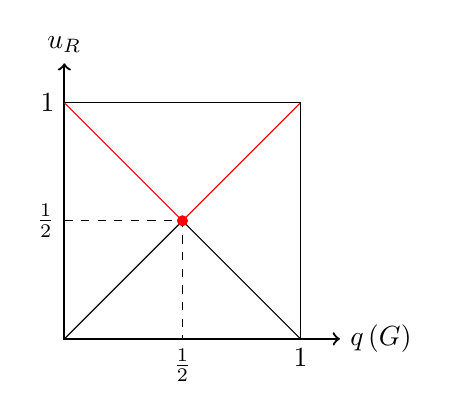
\begin{tikzpicture}
			\draw [<->,thick] (0,3.5) node (yaxis) [above] {$u_{R}$}
			|- (3.5,0) node (xaxis) [right] {$q\left( G\right) $};
			\draw (0,0) coordinate (a) -- (1.5,1.5) coordinate (m);
			\draw[red] (3,3) coordinate (d) -- (1.5,1.5) coordinate (m);
			\draw[red] (0,3) coordinate (b) -- (1.5,1.5) coordinate (m);
			\draw (3,0) coordinate (c) -- (1.5,1.5) coordinate (m);
			\draw[dashed] (yaxis |- m) node[left] {$\frac{1}{2}$}
			-| (xaxis -| m) node[below] {$\frac{1}{2}$};
			\draw (yaxis |- d) node[left] {$1$}
			-| (xaxis -| d) node[below] {$1$};
			\fill[red] (m) circle (2pt);
		\end{tikzpicture}
	\end{center}
	\pause
	$$A\left(q\right)=\begin{cases}
	\{acquit\} & if\ q\left(G\right)<\frac{1}{2} \\
	\alert{\{convict\}} & \alert{if\ q\left(G\right)=\frac{1}{2}} \\
	\{convict\} & if\ q\left(G\right)>\frac{1}{2}
\end{cases}$$
\end{frame}

\begin{frame}{Receiver的行动$\hat{a}\left( q\right) $}
	$$\hat{a}\left(q\right)=\begin{cases}
		\{acquit\} & if\ q\left(G\right)<\frac{1}{2} \\
		\alert{\{convict\}} & \alert{if\ q\left(G\right)\geq\frac{1}{2}} \\
	\end{cases}$$
	\begin{center}
		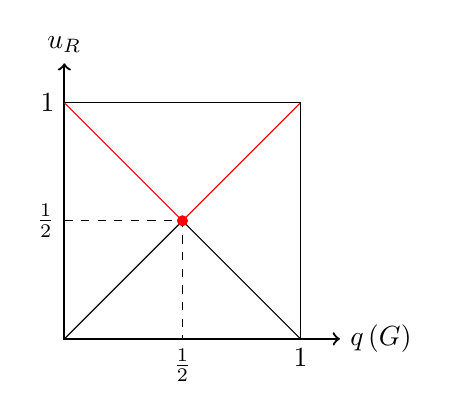
\begin{tikzpicture}
			\draw [<->,thick] (0,3.5) node (yaxis) [above] {$u_{R}$}
			|- (3.5,0) node (xaxis) [right] {$q\left( G\right) $};
			\draw (0,0) coordinate (a) -- (1.5,1.5) coordinate (m);
			\draw[red] (3,3) coordinate (d) -- (1.5,1.5) coordinate (m);
			\draw[red] (0,3) coordinate (b) -- (1.5,1.5) coordinate (m);
			\draw (3,0) coordinate (c) -- (1.5,1.5) coordinate (m);
			\draw[dashed] (yaxis |- m) node[left] {$\frac{1}{2}$}
			-| (xaxis -| m) node[below] {$\frac{1}{2}$};
			\draw (yaxis |- d) node[left] {$1$}
			-| (xaxis -| d) node[below] {$1$};
			\fill[red] (m) circle (2pt);
		\end{tikzpicture}
	\end{center}
\end{frame}

\begin{frame}{检察官的行动$\hat{v}\left(q\right)$}
	检察官(Sender)的行动需要根据法官行动反推收益函数。
	\begin{figure}
		\centering
		\begin{subfigure}[b]{0.45\textwidth}
			%\begin{adjustbox}{width=\linewidth} % rescale box
				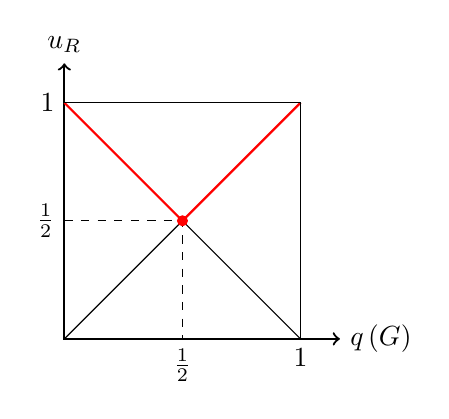
\begin{tikzpicture}
					\draw [<->,thick] (0,3.5) node (yaxis) [above] {$u_{R}$}
					|- (3.5,0) node (xaxis) [right] {$q\left( G\right) $};
					\draw (0,0) coordinate (a) -- (1.5,1.5) coordinate (m);
					\draw[red,thick] (3,3) coordinate (d) -- (1.5,1.5) coordinate (m);
					\draw[red,thick] (0,3) coordinate (b) -- (1.5,1.5) coordinate (m);
					\draw (3,0) coordinate (c) -- (1.5,1.5) coordinate (m);
					\draw[dashed] (yaxis |- m) node[left] {$\frac{1}{2}$}
					-| (xaxis -| m) node[below] {$\frac{1}{2}$};
					\draw (yaxis |- d) node[left] {$1$}
					-| (xaxis -| d) node[below] {$1$};
					\fill[red] (m) circle (2pt);
				\end{tikzpicture}
			%\end{adjustbox}       %
		\end{subfigure}%
		\hfill
		\begin{subfigure}[b]{0.45\textwidth}
			%\begin{adjustbox}{width=\linewidth} % rescale box
				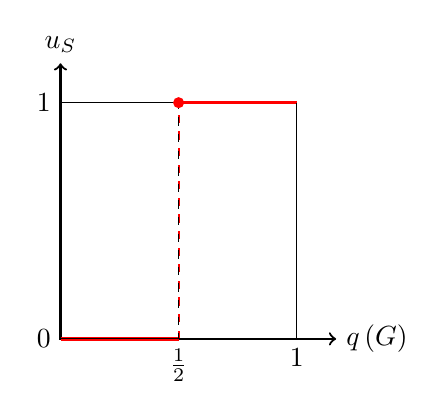
\begin{tikzpicture}
				\draw [<->,thick] (0,3.5) node (yaxis) [above] {$u_{S}$}
				|- (3.5,0) node (xaxis) [right] {$q\left( G\right) $};
				\draw[red,very thick] (0,0) coordinate (a) -- (1.5,0) coordinate (b);
				\draw[red,dashed,thick] (1.5,0) coordinate (c) -- (1.5,3) coordinate (d);
				\draw (0,3) coordinate (e) -- (1.5,3) coordinate(f);
				\draw[red,very thick] (1.5,3) coordinate (g) -- (3,3) coordinate (h);
				\draw (3,0) coordinate (i) -- (3,3) coordinate (j);
				\node (A) at (1.5,3) {};
				\node (B) at (3,3) {};
				\draw[dashed] (yaxis |- A) node[left] {1} -| (xaxis -| A) node[below] {$\frac{1}{2}$};
				\draw (yaxis |- i) node[left] {$0$}
				-| (xaxis -| i) node[below] {$1$};
				\fill[red] (d) circle (2pt);
				\end{tikzpicture}
			%\end{adjustbox}       %
		\end{subfigure}
	\end{figure}
	$$\hat{v}\left(q\right)=\begin{cases}
	0 & if\ q\left(G\right)<\frac{1}{2} \\
	\alert{1} & \alert{if\ q\left(G\right)\geq\frac{1}{2}} \\
\end{cases}$$
\end{frame}

\section{问题求解}

\subsection{最优劝说:福利与concavification}

\begin{frame}{进一步限制信息结构}
	信息结构$\pi : \Omega \to \Delta\left( S\right) $由\alert{有穷的}信号空间$S$和一组分布$ \left\lbrace \pi \left(\bullet | \omega \right)\right\rbrace_{\omega\in\Omega}  $构成。\\
	假设信息结构$\pi$能诱导出后验信念分布$\mu\in\Delta\left(\Delta\left( \Omega\right)\right) $,信息结构$\pi$的价值为信号发送者$R$的后验期望收益$E_{\mu}\left[\hat{v}\left(q\right)\right]  $\\
	此时,信息结构$\pi$的价值为$E_{\mu}\left[\hat{v}\left(q\right)\right]  $
\end{frame}

\begin{frame}{基准模型中的信息结构价值}
	\begin{itemize}
		\item[1] 完全披露\\
			如果检察官直接告知真实状态,均衡时检察官支付为0.3
		\item[2] 完全不披露\\
			如果检察官什么都不告知,均衡时检察官支付为0
	\end{itemize}
\end{frame}

\begin{frame}{定理1:从信息结构到后验信念}
	以下三个命题是等价的
	\begin{itemize}
		\item[1] 存在一个价值为$v^{*}$的信息结构
		\item[2] 存在一个信号实现空间$ S \subset A$(信号实现空间是行动空间子集)、价值为$v^{*}$的信息结构
		\item[3] 存在一个贝叶斯可信的(Bayes-plausible)后验信念分布$\mu$,使信号发送者期望收益$E_{\mu}\left[\hat{v}\left(q\right)\right] $等于$v^{*}$
	\end{itemize}
	贝叶斯可信:先验分布等于后验分布的期望$p=E_{\mu} \left[q\right]$\\
	分离引理:给定先验信念$ p\in \Delta \left( \Omega \right)$,当且仅当后验信念满贝叶斯可信,先验信念可以通过某一信息结构诱导出后验信念的分布。\\~\\
	选择信息结构、选择行动建议和选择后验分布是等价的。\\

\end{frame}

\begin{frame}{发送者能从劝说中获益吗?}
	推论1:发送者能从劝说中获益。\\
	当且仅当存在贝叶斯可信后验分布$\mu\in\Delta\left(\Delta\left( \Omega\right)\right) $,使$E_{\mu} \left[\hat{v}\left(q\right)\right]>\hat{v}\left(p\right)$,信息发送者能从劝说中获益,即。$ v^{*}>\hat{v}\left(p\right) $\\
	最优信息结构的价值是最优化后验分布问题:
	$$\max_{\mu} E_{\mu} \left[\hat{v}\left(q\right)\right]$$
	$$s.t.\  \underset{bayes-plausible}{p=E_{\mu} \left[q\right]}$$
	即给定先验分布$q$,在贝叶斯可信$ p=E_{\mu} \left[q\right] $的约束下,选择后验分布$ \mu $最大化信息结构的价值$\hat{v}\left(q\right) $。\\
	$\hat{v}$不是连续的,但是上半连续的,加之$\mu$是紧集,最优化问题恒有解。(KG2011,Proposition 6)\\~\\

\end{frame}

\begin{frame}{concavification}
	回顾$\hat{v}:\ \Delta\left(\Omega \right)  \to  \mathbb{R}$的图像:
	$$C\left(\hat{v}\right) = \left\lbrace \left(q,\hat{v}\left(q\right)\right) | q\in \Delta\left(\Omega\right)  \right\rbrace$$
	定义$\hat{v}$的凹闭包(concave closure)$V:\Delta\left(\Omega \right)  \to  \mathbb{R}$:
	$$V\left(q\right) = \sup \left\lbrace z\in \mathbb{R} | \left(q,z\right)\in \text{conv} \ C\left(v\right) \right\rbrace$$
	此时,$V\left(q\right)$是盖在$\hat{v}$上最小的凹函数。
\end{frame}
\begin{frame}{凹闭包与最大福利的直觉}
	\begin{center}
		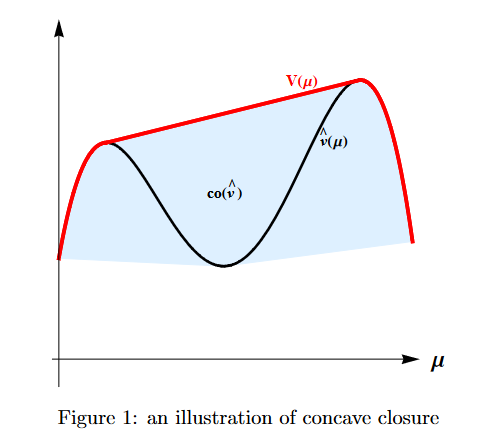
\includegraphics[width=0.5\linewidth]{pic/fig1.png}
	\end{center}
	如果$\left(q,v\right) \in \text{conv}\ C\left(\hat{v}\right)$,即点$\left(q,v\right)$在$C\left(\hat{v}\right)$图像的凸包内部,存在后验信念$\mu \in \Delta\left(\Delta \left(\Omega \right)\right)$,满足$q=E_{\mu}\left[q^{1}\right]$和$v=E_{\mu}\left[\hat{v}\left(q\right)\right]$\\
		引理2:最优信息结构的价值为$V\left(p\right)$
\end{frame}

\begin{frame}{案例}
		\begin{figure}
		\centering
		\begin{subfigure}[b]{0.45\textwidth}
			%\begin{adjustbox}{width=\linewidth} % rescale box
			\begin{tikzpicture}
				\draw [<->,thick] (0,3.5) node (yaxis) [above] {$u_{S}$}
				|- (3.5,0) node (xaxis) [right] {$q\left( G\right) $};
				\draw[red,very thick] (0,0) coordinate (a) -- (1.5,0) coordinate (b);
				\draw[red,dashed,thick] (1.5,0) coordinate (c) -- (1.5,3) coordinate (d);
				\draw (0,3) coordinate (e) -- (1.5,3) coordinate(f);
				\draw[red,very thick] (1.5,3) coordinate (g) -- (3,3) coordinate (h);
				\draw (3,0) coordinate (i) -- (3,3) coordinate (j);
				\node (A) at (1.5,3) {};
				\node (B) at (3,3) {};
				\draw[dashed] (yaxis |- A) node[left] {1} -| (xaxis -| A) node[below] {$\frac{1}{2}$};
				\draw (yaxis |- i) node[left] {$0$}
				-| (xaxis -| i) node[below] {$1$};
			\end{tikzpicture}
			%\end{adjustbox}       %
		\end{subfigure}%
		\hfill
		\begin{subfigure}[b]{0.45\textwidth}
			%\begin{adjustbox}{width=\linewidth} % rescale box
			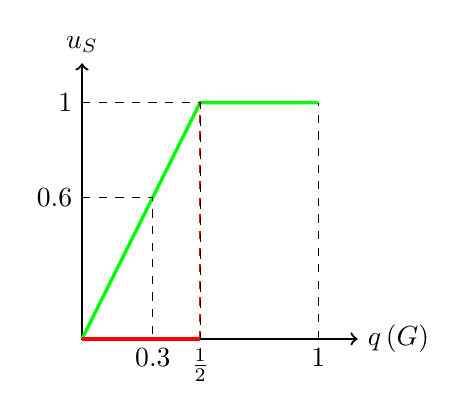
\begin{tikzpicture}
				\draw [<->,thick] (0,3.5) node (yaxis) [above] {$u_{S}$}
				|- (3.5,0) node (xaxis) [right] {$q\left( G\right) $};
				\draw[green,very thick] (0,0) -- (1.5,3) -- (3,3);
				\draw[red,very thick] (0,0) coordinate (a) -- (1.5,0) coordinate (b);
				\draw[red,dashed,thick] (1.5,0) coordinate (c) -- (1.5,3) coordinate (d);
				\node (A) at (1.5,3) {};
				\node (B) at (3,3) {};
				\draw[dashed] (3,0) -- (3,3);
				\draw[dashed] (yaxis |- A) node[left] {1} -| (xaxis -| A) node[below] {$\frac{1}{2}$};
				\draw[dashed] -| (xaxis -| B) node[below] {$1$};
				\pause;
				\node (C) at (0.9,1.8) {};
				\draw[dashed] (yaxis |- C) node[left] {0.6} -| (xaxis -| C) node[below] {0.3};
			\end{tikzpicture}
			%\end{adjustbox}       %
		\end{subfigure}
	\end{figure}

\end{frame}
\begin{frame}{补充结论:$\hat{v}$函数性质与获益}
	KG2011 Propositon 8:\\
	对于任意先验概率$p\in \text{Int} \ \Delta\left(\Omega\right)$:
	\begin{itemize}
		\item[1] 如果$\hat{v}$严格凹,$\hat{v}=V$,信号发送者不能从劝说中获益。
		\item[2] 如果$\hat{v}$严格凸,信号发送者完全披露时获益最大。
		\item[3] 如果$\hat{v}$为凸函数(非凹函数),信号发送者能从劝说中获益。
	\end{itemize}
\end{frame}


\section{把信息设计转化成最优化问题}

\subsection{广义信息设计}

\begin{frame}{用博弈论的思路探讨信息设计}
	一个完整的博弈$G$需要包括至少三部分:
	\begin{itemize}
		\item[1] 参与者$i\in I$、参与者行动$A_{i}$和行动的效用$u_{i}: \ A\times\Omega\to\mathbb{R}$。
		\item[2] 状态(不确定、不能对所有人公开)$\omega\in\Omega$
		\item[3] 状态发生的先验概率分布(先验信念)$p\in \text{Int} \left(\Delta\left(\Omega\right)\right)$
	\end{itemize}
	$$G=\left(\left(A_{i},u_{i}\right),\Omega,p\right)$$
	博弈结果$v\in\Delta\left(A\times\Omega\right)$:行动与状态的联合分布概率\\
	信息结构:$T=\left(\left(S_{i}\right)_{i\in I},\tau\right)$
	\begin{itemize}
		\item[$S_{i}$] :私人信号空间,只有参与人自己知道
		\item[$ S $] :信号组合,$S=S_{1}\times\dots S_{|I|}$
		\item[$ \tau $] :共同先验信念,$\tau \in \Delta\left(S\times\Omega\right)$,某一信息结构同一状态下的先验信念$p\left(\omega\right)$必须与关于状态的边缘分布$\sum_{S}\ \tau\left(S,\omega\right)$一致。
		
	\end{itemize}
\end{frame}

\begin{frame}{法官与检察官:博弈语言}
	\begin{itemize}
		\item[] $I=\left\lbrace \text{法官} \right\rbrace$
		\item[] $A=\left\lbrace \text{判无罪(acquit),判有罪(convict)} \right\rbrace$
		\item[] $\Omega=\left\lbrace G,I\right\rbrace$
		\item[] $p\left(G\right)=0.3, \ p\left(I\right)=0.7$
		\item[] $u\left( acquit,I\right) =u\left( convict,G\right)=1 \text{;} $
		\item[] $u\left( acquit,G\right) =u\left( convict,I\right)=0$
		\item[] $S=\left\lbrace g,i\right\rbrace$
		\item[] description
	\end{itemize}
	信息结构$T=\left(S,\tau\right)$满足
	$$\tau\left(g,G\right)=\ $$
\end{frame}

\begin{frame}
	内容...
\end{frame}
\subsection{贝叶斯纳什均衡:为什么是$\frac{3}{7}$和$\frac{4}{7}$?}



\section{中文例子}

\begin{frame}{问题导入}
	治理失灵现象普遍存在,但治理失灵被内生于治理体系中。\\~\\
	\begin{itemize}
		\item 基层政府的选择性执行
		\item 政策治理的变通行为
		\item 消极执行与运动式执行 \\~\\
	\end{itemize}
	
	“非正式行为”为什么在上级政府具有纠偏能力时也会被制度化?\\
	
\end{frame}

\subsection{基准模型设定}

\begin{frame}
	假定上级政府$U$和下级政府$D$政策集为$X\in\{a,b\}$\\
	上级政府负责制定政策,下级政府负责执行政策。\\
\end{frame}
\subsection{严格执行}

\subsection{变通执行}



\end{document}